\chapter{Esquema TN}
Es un esquema donde las masas están conectadas o bien al cable de protección o al neutro. Los defectos se ven en las protecciones como cortocircuitos.
\section{Esquema TN – S}
\begin{figure}[H]
	\centering
	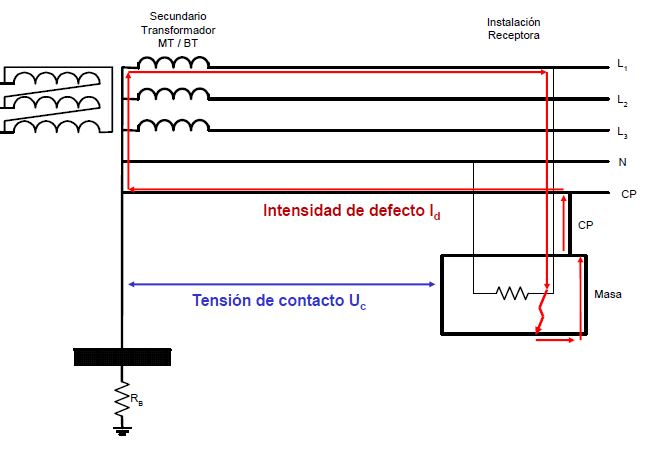
\includegraphics[width=0.7\linewidth]{Images/29}
	\label{fig:29}
\end{figure}

Con su circuito equivalente:
\begin{figure}[H]
	\centering
	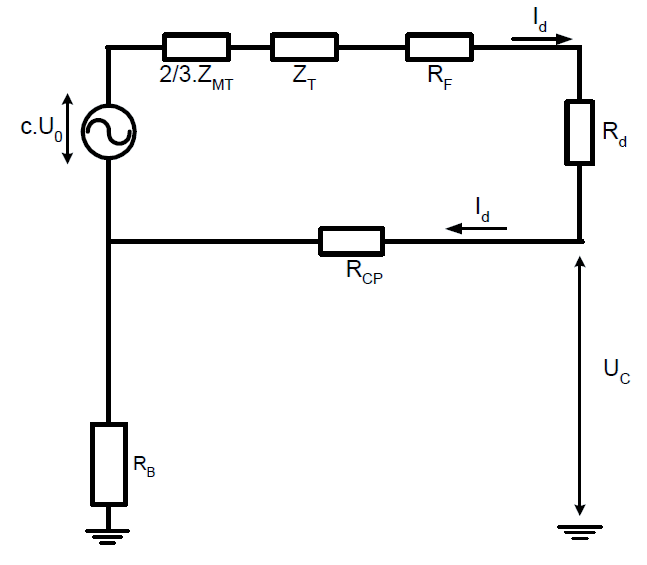
\includegraphics[width=0.5\linewidth]{Images/30}
	\label{fig:30}
\end{figure}

Se puede simplificar el cálculo de cortocircuito tal como se estudió en el tema 2 para un \textbf{cortocircuito fase-neutro} o monofásico. No obstante, si se puede es mejor el cálculo exacto. \textbf{Se debe disparar en caso de defecto mediante un interruptor automático.}
\begin{equation}
	I_d=0,8\dfrac{U_0}{Z_s}
\end{equation}
\begin{equation}
	U_C=R_{CP}\cdot I_d
\end{equation}
\section{Esquema TN – C}
\begin{figure}[H]
	\centering
	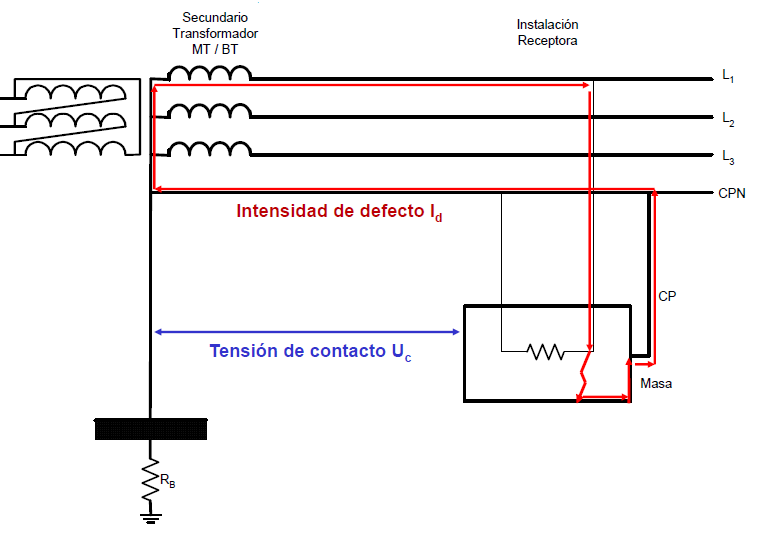
\includegraphics[width=0.7\linewidth]{Images/31}
	\label{fig:31}
\end{figure}

Con su circuito equivalente:
\begin{figure}[H]
	\centering
	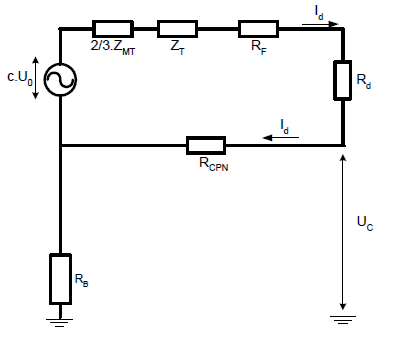
\includegraphics[width=0.7\linewidth]{Images/32}
	\label{fig:32}
\end{figure}

El cálculo es similar al de un esquema TN-S
\section{Condiciones de protección}
\begin{itemize}
	\item Todas las masas de los equipos eléctricos protegidos por un mismo dispositivo de
	protección deben estar unidas por un conductor de protección (CP o CPN) a la toma
	de tierra de la alimentación (también denominada fuente)
	\item Puede ser necesaria una puesta a tierra múltiple, en puntos repartidos con
	regularidad, para asegurarse que el potencial del conductor de protección se
	mantiene, en caso de fallo, lo más próximo posible al de tierra
	\item Por la razón anterior, se recomienda conectar el conductor de protección a tierra en
	el punto de entrada de cada edificio
	\item Las características de los dispositivos de protección y las secciones de los
	conductores se eligen de manera que, si se produce en un lugar cualquiera un fallo,
	de impedancia despreciable, entre un conductor de fase y el conductor de
	protección o una masa, el corte automático se efectúe en un tiempo igual, como
	máximo, al valor especificado, y se cumpla la condición siguiente:
	\begin{equation}
		Z_s\cdot I_a < U_F
	\end{equation}
	Donde $Z_s$ es la impedancia del bucle de defecto, $I_a$ la corriente de apertura de la protección y $U_F$ la tensión de fase
	
	\item  Condición de protección de tiempo:
	\begin{table}[H]
		\centering
		\renewcommand{\arraystretch}{1.5}
		\setlength{\tabcolsep}{8pt}
		\begin{tabular}{|c|c|}
			\hline
			\textbf{$U_0$ (V)} & \textbf{Tiempo de interrupción c.a. (s)} \\ \hline
			$120 < U_0 \leq 230$ & 0,4 \\ \hline
			$230 < U_0 \leq 400$ & 0,2 \\ \hline
			$U_0 > 400$ & 0,1 \\ \hline
		\end{tabular}
		\label{tabla:tiempo_interrupcion}
	\end{table}
	Los valores anteriores deben aplicarse siempre y cuando la corriente no supere:
	\begin{itemize}
		\item 63 A con una o más tomas de corriente
		\item 32 A alimentando solo receptores conectados de forma fija
	\end{itemize}
	En circuitos de distribución y para circuitos distintos a los indicados, retardos de hasta 1 s
	pueden ser suficientes para asegurar selectividad.
\end{itemize}

En esencia, debe cumplirse que los automáticos disparen contra cortocircuitos cuando ocurra el defecto.

\subsection{Requisitos adicionales}
\begin{itemize}
	\item El neutro se conectará a tierra cada 200 m
	\item La resistencia de puesta a tierrra del neutro sera menor a $5\Omega$ en el CT y en los últimos 200 m de cualquier derivación
	\item La resistencia global de tierra, de todas las tomas del neutro, será menor o igual a $2\Omega$
	\item En el esquema TN-C las masas de las instalaciones receptoras deben conectase al
	conductor de neutro mediante conductores de protección
	\item En el esquema TN-C no se pueden utilizar interruptores diferenciales. En el esquema TN-S se pueden utilizar interruptores diferenciales.
	\item Cuando se instale un interruptor diferencial en un esquema TN-C-S no debe utilizarse un conductor
	CPN aguas abajo del diferencial (si se conecta neutro con masa no dispara el interruptor)
\end{itemize}
\section{Consideraciones importantes}
Un defecto de aislamiento entre neutro N y conductor de protección CP
transforma el esquema TN-S en TN-C. 
\newline

Esto implica que una parte de la corriente de neutro pasa de forma permanente por el
CP y, por tanto, por las estructuras metálicas del edificio a las que esté conectado el CP,
con dos consecuencias:
\begin{itemize}
	\item La equipotencialidad del CP no está asegurada
	(una pequeña caída de tensión puede perturbar
	el funcionamiento de los sistemas informáticos)
	\item La circulación de corriente por el interior de
	estructuras aumenta el riesgo de incendio
\end{itemize}

Se puede solucionar mediante señalización mediante protección diferencial con sensibilidad de
0,5 A o superior para detectar bajadas de corriente en el neutro
\section{Longitud máxima protegida}
Se calcula la resistencia máxima que pueden tener los conductores en el caso de que la intensidad de defecto sea la de actuación:
\begin{equation}
	I_d=\dfrac{0,8 U_F}{R_F+R_{CP}}
\end{equation}
\begin{equation}
	R=\rho\dfrac{L}{S}
\end{equation}
\section{Casos con impedancia del bucle muy elevada}
Para los casos en los que el interruptor automático no garantice la
protección contra contactos indirectos en toda la longitud de la
instalación, existen las siguientes soluciones:
\begin{itemize}
	\item Interruptor automático de regulación magnética más baja (si la carga
	necesita corrientes de conexión elevadas esta solución no es válida)
	\item Aumentar la sección de los conductores de protección, de las fases, o
	de ambos
	\item Realizar una conexión equipotencial complementaria a la parte de la
	instalación no protegida por el dispositivo de corte (instalación supervisada)
	\item Instalar un interruptor diferencial en cabecera del circuito terminal a proteger
	que garantice la protección de personas frente a contactos indirectos
\end{itemize}